\documentclass[runningheads,a4paper]{llncs}

\usepackage[utf8]{inputenc}
\usepackage[spanish,activeacute]{babel}
\setcounter{tocdepth}{3}
\usepackage{graphicx}
\usepackage{subfigure}
\usepackage{url}

\newcommand{\keywords}[1]{\par\addvspace\baselineskip
\noindent\keywordname\enspace\ignorespaces#1}

\providecommand{\tabularnewline}{\\}


\begin{document}

%%%%%%%%%%%%%%%%%%%%%%%%%%%%%%%   TITLE   %%%%%%%%%%%%%%%%%%%%%%%%%%%%%%%

\title{Factores de influencia por género en la elección de Grados relacionados con la Tecnología}

%%%%%%%%%%%%%%%%%%%%%%%%%%%%%%%   AUTHORS   %%%%%%%%%%%%%%%%%%%%%%%%%%%%%%%

\author{Paloma de las Cuevas, Maribel García Arenas \inst{1}}
\authorrunning{P. de las Cuevas et al.}

\institute{Dept. de Arquitectura y Tecnología de Computadores, Universidad de Granada}

\maketitle

%
%%%%%%%%%%%%%%%%%%%%%%%%%%%%%%%%%   ABSTRACT   %%%%%%%%%%%%%%%%%%%%%%%%%%%%%%%%%
%
\begin{abstract}
Ante la tendencia decreciente de la matriculación de mujeres en las ingenierías, y a la necesidad no cubierta desde Europa de incorporación de ingenieros e ingenieras al mundo laboral, se plantea un problema a resolver, que es cómo hacer las ingenierías más atractivas para los y las adolecentes.
Se debe hacer esta distinción entre chicos y chicas puesto que los factores por los que finalmente no estudian una ingeniería son distintos. Esto quiere decir que a ambos sexos les afecta una serie de factores derivados del entorno, de su percepción hacia ellos mismos y hacia los diversos aspectos de las ingenierías, pero que además el hecho de que existan una serie de estereotipos afecta a las chicas por separado.
En este Trabajo Fin de Máster se presenta un análisis de los factores de influencia, y en profundidad de los factores de género, que afectan a la decisión de escoger una carrera, en este caso particularizando en las ingenierías.
Además, se ha observado e identificado la influencia de dichos factores en un contexto de centro secundaria en Granada, en el que se han realizado una serie de encuestas a alumnos de Educación Secundaria Obligatoria, Bachillerato, y Ciclos Formativos relacionados con la Tecnología y la Informática.

\keywords{...}
\end{abstract}

%%%%%%%%%%%%%%%%%%%%%%%%%%%%%%%   INTRODUCTION   %%%%%%%%%%%%%%%%%%%%%%%%%%%%%%%
%
\section{Introducción}
\label{sec:intro}

Ante la creciente necesidad de ingenieros e ingenieras en Europa \cite{gago2004europe}, los gobiernos europeos se han movilizado para intentar que crezca el interés por las ingenierías en los niveles de las enseñanzas medias \cite{Kearney2014}. Lo que es más, según la OECD\footnote{Organisation for Economic Co-operation and Development} \cite{OECD2006}, la representación femenina en carreras relacionadas con la ciencia y la tecnología permanece debajo del 40\%. En lo referente a España, según vemos en la Figura \ref{fig:ing_total}, la media de mujeres en las ``Enseñanzas Técnicas'' - entre las que se incluyen Ingeniería Informática e Ingeniería de Telecomunicaciones - es apenas de un 31\%. El cambio al Plan Bolonia \cite{fernandez2009plan} no ha mejorado esta situación, sino que, como se visualiza en la Figura \ref{fig:grado_total}, la media de mujeres matriculadas en Grados de Enseñanzas Técnicas cae y no llega al 25\%.

\begin{figure}[ht]
        \centering
        \subfigure[\scriptsize{Ingenierías del plan antiguo, entre las que se incluyen Ingeniería Informática e Ingeniería de Telecomunicaciones. \textit{(*) Datos no disponibles en \cite{datos::uni}.}}]{
                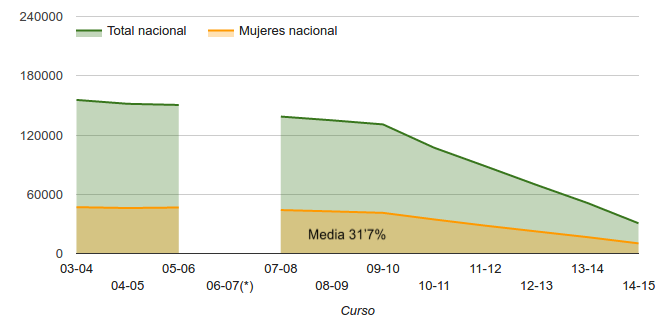
\includegraphics[width=0.8\textwidth,keepaspectratio]{Bitmap/ing_total.png}
                \label{fig:ing_total}
        }
        \subfigure[\scriptsize{Grados de Ingenierías o Enseñanzas Técnicas.}]{
                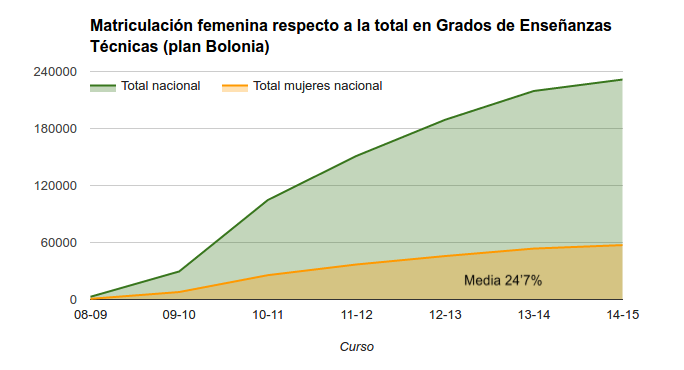
\includegraphics[width=0.8\textwidth,keepaspectratio]{Bitmap/grado_total.png}
                \label{fig:grado_total}
        }
        \caption{{\footnotesize Evolución de la matriculación de mujeres en Enseñanzas Técnicas en Universidades tanto públicas como privadas. Fuente de datos: \cite{datos::uni}.}}\label{fig:datos_total}
\end{figure}

El propósito de este artículo es el de clarificar si los factores encontrados en la literatura son válidos para un instituto de la provincia de Granada, en el cual se ha realizado un estudio mediante encuestas a estudiantes de 3º y 4º de E.S.O.\footnote{Educación Secundaria Obligatoria}, 1º y 2º de Bachillerato, y Ciclos Formativos. Para ello, en primer lugar se identificarán en la sección \ref{sec:factores} los factores que diversos estudios encontrados en la literatura han identificado como determinantes para la elección de ingenierías. Después, en la Sección \ref{sec:EdA} se estudiará el Estado del Arte según las propuestas existentes para tratar de equilibrar las cifras en cuanto cantidad de mujeres matriculadas en Enseñanzas Técnicas. La Sección \ref{sec:metodologia} detalla el contexto en el que se han hecho las encuestas, además de las razones por las que se han escogido cada una de las preguntas, así como las fuentes. Por último, en la Sección \ref{sec:resultados} se analizan los resultados obtenidos, según los tres bloques de Secundaria, Bachillerato y Ciclos Formativos, para en la Sección \ref{sec:conclusiones} ofrecer las conclusiones sobre este estudio y unas nociones sobre el trabajo futuro.

\section{Factores de influencia identificados en la literatura}
\label{sec:factores}

\section{Estado del Arte}
\label{sec:EdA}

\section{Metodología}
\label{sec:metodologia}

\section{Resultados}
\label{sec:resultados}

\section{Conclusiones}
\label{sec:conclusiones}

...


\section*{Agradecimientos} 

...


%
%Hidden for double-blind review


\bibliographystyle{splncs03}
\bibliography{eleccion_grado}


\end{document}
